\textbf{Investiga y explica brevemente de qué se trata el juego de la imitación de Alan M. Turing. Cita tus fuentes (0.5 pt.).}

También conocido como la prueba de Turing, es un experimento mental propuesto por Alan M. Turing en su artículo \textit{Computing Machinery and Intelligence}. La idea es que, para probar la consciencia o su ausencia en las máquinas, se sitúan una máquina, una persona y una segunda persona que actuará como juez; de esta forma, mediante preguntas y respuestas, el mediador, representado en la figura 'C', debe determinar quién es la computadora y quién es la persona. Si el sistema es capaz de engañar a un alto porcentaje de los jueces, se le considera que ha pasado la prueba de Turing. \vspace{.3cm}

\cite{turing1950computing}

\begin{figure}[h]
    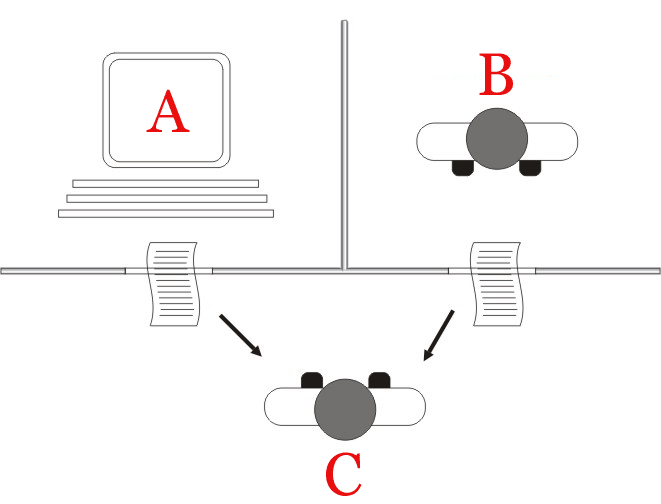
\includegraphics[width=10cm]{src/Img/Turing_test_diagram.png}
    \centering
    \caption{\cite{testTuring}}
\end{figure}

Aunque el hecho de que el sistema pase el test, en realidad, no nos indica más que su capacidad para comunicarse de manera coherente. Aun así, es altamente probable que nos encontremos ante un escenario similar al experimento del cuarto chino de John Searle, en el que la computadora realmente no tiene idea de lo que está haciendo, pero es capaz de engañar al mediador mediante tácticas inteligentes, generalmente basadas en métodos estadísticos y neuronales. \vspace{.3cm}
